
\subsection{The conditional average}
\tb{re-write with the interface Indicator function propoability and stuffs}
The first step is to introduce the relation between particle averaged field and \textit{single-particle} conditionally-averaged field.
For instance, let us take the example of the drag force term. 
Form the definition of the particle-average \ref{eq:p_avg} we write,
\begin{align}
    \pSavg{\bm\sigma_f^0\cdot\textbf{n}}[\textbf{x},t]
    &= \int \sum_{\alpha=1}^N \delta(\textbf{x}-\textbf{x}_\alpha[t; \FF])
    \int_{\Gamma_\alpha(t,\FF)}
    \bm\sigma_f^0\cdot\textbf{n}[\textbf{y},t;\FF]
    d\Gamma(\textbf{y}) d\PP
\end{align}
By writing this integral explicitly, we want to emphasize that the particle-averaged quantity is evaluated at the point \textbf{x}, while the integration over the surface of the particles $\alpha$ is carried out over the surface with the integration parameter $\textbf{y}$.
Therefore, we may enlarge the domain of integration from $\Gamma_\alpha$ to $\mathbb{R}^3$ by multiplying $\bm\sigma_f^0\cdot\textbf{n}(\textbf{r},t;\FF)$ with $\delta(|\textbf{y} - \textbf{x}_\alpha(t,\FF)| - a)$. 
It reads, 
\begin{equation}
    \pSavg{\bm\sigma_f^0\cdot\textbf{n}}[\textbf{x},t]
    = 
    \int_{\mathbb{R}^3}
    \int
     \sum_{\alpha=1}^N 
     \delta(\textbf{x}-\textbf{x}_\alpha(t; \FF))
    \delta(|\textbf{y} - \textbf{x}_{\alpha}(t;\FF)|-a)
    (\bm\sigma_f^0\cdot\textbf{n})[\textbf{y},t;\FF]
    d\PP
    d\textbf{y}
\end{equation}
Note that this definition is only valid for identical spherical particles of radius $a$. 
Due to the presence of $\delta(\textbf{x}-\textbf{x}_\alpha(t; \FF))$, this expression is non-zero only when $\textbf{x} = \textbf{x}_\alpha(\FF,t)$. 
Also, we can introduce the conditional average on the velocity of the particle by noticing that, 
\begin{equation*}
    \int_{\mathbb{R}^3} \delta(\textbf{c} - \textbf{u}_\alpha(\FF,t)) d\textbf{c} = 1. 
\end{equation*}
Taking in account the preceding remarks we are able to write
\begin{equation}
    \pSavg{\bm\sigma_f^0\cdot\textbf{n}}[\textbf{x},t]
    =
    n_p(\textbf{x})
    \int_{\mathbb{R}^3}
    \int_{|\textbf{x}-\textbf{y}|=a}
    \bm\sigma_f^1[\textbf{y},t;\textbf{x},\textbf{c}] \cdot \textbf{n}
    d\textbf{y}
    d\textbf{c}
    \label{eq:conditionally_averaged}
\end{equation}
where, 
\begin{equation*}
    \bm\sigma^1_f[\textbf{y},t;\textbf{x},\textbf{c}] n_p(\textbf{x},\textbf{c})
    =
    \avg{\delta_\alpha \bm\sigma^0_f}[\textbf{y},t;\textbf{x},\textbf{c}]
    = 
    \int 
    \sum_\alpha^N 
    \delta(\textbf{x} - \textbf{x}_\alpha(\FF,t))
    \delta(\textbf{c} - \textbf{u}_\alpha(\FF,t))
    \bm\sigma_f^0[\textbf{y},t;\FF]
    d\PP
\end{equation*}
is the \textit{single-particle} conditionally-averaged local stress of the continuous phase knowing that interface of the particle at $\textbf{x}$ is  present in \textbf{y}. 
In other world $\bm\sigma^1_f$ is the mean fluid phase stress evaluated at $\textbf{y}$ and time $t$ on every configuration where a particle is present at $\textbf{x}$. 
And $n_p(\textbf{x})$ is the number density but evaluated at $\textbf{x}$.
In light of \ref{eq:conditionally_averaged} we made the link between particle-average and the integral of a \textit{single-particle} conditionally-averaged quantity. 
Note that all quantities denoted with the superscript $^1$ refer to \textit{single-particle} conditionally-averaged  quantities.  
Therefore, it is implicit that these quantities are evaluated at $\textbf{y}$ and $t$ and conditionally on $\textbf{x}$. 

At some point it will also be useful to express continuous phase averaged quantities, i.e. $\avg{\chi_k f_k^0}$  in terms of one  \textit{single-particle} conditionally-averaged fields. 
Two examples are the Reynolds stress $\avg{\chi_f \textbf{u}_f'\textbf{u}_f'}$ and the fluid phase dissipation $\avg{\chi_f\sigma_f^0:\grad \textbf{u}_f^0}$ that appear in \ref{eq:dt_hybrid_rhou_f} and \ref{eq:dt_hybrid_k1}, respectively.  
To proceed one must first note that, 
\begin{equation}
    \frac{1}{N}\sum_\alpha 
    \int_{\mathbb{R}^3}
    \int_{\mathbb{R}^3}
    \delta(\textbf{y}-\textbf{x}_\alpha)
    \delta(\textbf{c}-\textbf{u}_\alpha)
    d\textbf{x}
    d\textbf{c}
    = 1
\end{equation}
where $N$ is the total number of particle in the flow. 
Using this relation one may re-formulate the ensemble average of a continuous phase quantity as 
\begin{equation}
    f_f[\textbf{x},t]
    = 
    \frac{1}{N}
    \int_{\mathbb{R}^3}
    \int_{\mathbb{R}^3}
    f_k^1[\textbf{x},t|\textbf{y},\textbf{c}]  P_1[\textbf{y},\textbf{c}|\textbf{x},t] 
    d\textbf{y} 
    d\textbf{c}
    \label{eq:conditional_averaged_fluid}
\end{equation}
where,
\begin{equation*}
    f_k^1[\textbf{x},t|\textbf{y},\textbf{c}] P_1[\textbf{y},\textbf{c}|\textbf{x},t] \phi_k[\textbf{x},t]
    =     
    \int
    \sum_\alpha^N 
    \delta(\textbf{y}-\textbf{x}_\alpha)
     \delta(\textbf{c}-\textbf{u}_\alpha)
    \chi_k
    f^0_k[\textbf{x},t;\FF]
    d\PP.
\end{equation*}
In this expression $f_f^1[\textbf{x},t;\textbf{y},\textbf{c}]$ is the average of the local quantity $f_f^0$ evaluated at $\textbf{x}$ and time $t$ conditionally on the presence of a particle center of mass at $\textbf{y}$ with center of mass velocity $\textbf{c}$. 
% Similarly, $\phi_f^1[\textbf{x},t;\textbf{y},\textbf{c}]$ is the fluid phase volume fraction at \textbf{x} and time $t$, conditionally on the presence of a particle at $\textbf{y}$ with velocity \textbf{c}. 
Similarly, $P_1[\textbf{y},\textbf{c};\textbf{x},t]$ is the probability density of finding a particle center of mass within the infinitesimal volume $d\textbf{y}$ around $\textbf{y}$ with a center of mass velocity ranging between the interval $d\textbf{c}$ around $\textbf{c}$, knowing that the point \textbf{x} is occupied by the continuous phase. 
Note that this derivation is consistent with (2.21) and (2.22) of \citet{zhang1994ensemble} with $K = 1$. 


% In case of potential or stokes flow the linearity of the equation permits us to write, 
% \begin{equation*}
%     f_f^1(\textbf{x},t|\textbf{y})
%     = 
%     \sum_i
%     f_{f_i}^1(\textbf{x},t|\textbf{y})
%     + f_{f_0}^1(\textbf{x},t)
% \end{equation*}
% where $f_{f_i}^1$ is the averaged disturbance fields produced by the particle $i$ at $\textbf{y}$ on $f_f^1$ and $f_{f_0}^0$ is the undisturbed background field.
% Using this decomposition into \ref{conditional_averaged_fluid} yield a second definition for the fluid phase average 
% \begin{equation*}
%     f_f[\textbf{x},t]
%     = 
%     \frac{1}{N}
%     \sum_i
%     \int_{\mathbb{R}^3}
%     \int_{\mathbb{R}^3}
%     f_{k_i}^1[\textbf{x},t|\textbf{y},\textbf{c}]  
%     P_1[\textbf{y},\textbf{c}|\textbf{x},t] 
%     d\textbf{y} 
%     d\textbf{c}
%     + 
%     f_{k_0}[\textbf{x},t]  
% \end{equation*}
% assuming that the contribution from each particles is statistically equivalent we find 


In practice \ref{eq:conditional_averaged_fluid} cannot be used since the number of particle $N$ is unknown. 
Therefore, we follow a method similar to \citet{batchelor1972sedimentation} and assume linearity of the local scale equations. 
Therefore, we stipulate that $f_f^0(\textbf{x},t;\FF)$ can be subdivided into $N$ contribution, namely  
\begin{equation}
    f_f^0(\textbf{x},t;\FF)
    = 
    \sum_i
    f_{f_i}^0(\textbf{x},t;\FF)
    + f_{f_0}^0(\textbf{x},t;\FF)
\end{equation}
where $f_{f_i}^0(\textbf{x},t;\FF)$ is the disturbance fields produced by the particle $i$ on $f_f^0$ and $f_{f_0}^0$ is the undisturbed background flow. 
This of course implies that $f_f^0 = 0$ in the absence of particle in the flow. 
Under this very restrictive hypothesis we can write, 
\begin{equation}
    \avg{\chi_ff_f^0}[\textbf{x},t]
    = 
    \sum_i
    \avg{\chi_f f_{f_i}^0(\textbf{x},t;\FF)}
    = 
    \int_{\mathbb{R}^3} 
    \avg{
        \sum_i
    \chi_f f_{f_i}^0(\textbf{x}_\alpha + \textbf{r},t;\FF) \delta(\textbf{x} - \textbf{x}_\alpha - \textbf{r})}d\textbf{r}
\end{equation}
assuming that \textbf{r} is relatively small compared to the macroscale we may write $\delta(\textbf{x} - \textbf{x}_\alpha - \textbf{r}) =\delta(\textbf{x} - \textbf{x}_\alpha) - \textbf{r}\cdot \grad\delta(\textbf{x} - \textbf{x}_\alpha)+ \ldots$
\begin{equation}
    \avg{\chi_ff_f^0}[\textbf{x},t]
    = 
    \int_{\mathbb{R}^3} 
    \phi_f^1
    f_{f_i}^1(\textbf{x}+ \textbf{r}| \textbf{x})
    n_p(\textbf{x}) 
    d\textbf{r}
    +
    \phi_f f_{k_0}^1[\textbf{x},t]  
\end{equation}
with, 
\begin{equation*}
    \phi_f^1 f_{f_i}^1[\textbf{x}+ \textbf{r}| \textbf{x}]n_p(\textbf{x}) 
    = 
    \int{
    \sum_i
    \chi_f f_{f_i}^0(\textbf{x}_\alpha + \textbf{r},t;\FF) \delta(\textbf{x} - \textbf{x}_\alpha)
    }d\PP
\end{equation*}
$f_{f_i}^1[\textbf{x}+ \textbf{r}| \textbf{x}]$ is the averaged value of $f_{f_i}^0$ at $\textbf{x}+\textbf{r}$ knowing a particle is at \textbf{x} and that the point $\textbf{x}+\textbf{r}$ is occupied by the continuous phase. 
Thus, in this definition $f_{f_i}^1$ is the averaged value of the disturbance fields produced by the particle in $\textbf{x}$ only.
At order one in the particle volume fraction $\phi_f^1 = \phi_f$ when $|\textbf{x}-\textbf{y}|>a$ and $à$ otherwise thus, 
\begin{equation}
    \avg{\chi_f f_f^0}[\textbf{x},t]
    = 
    \phi_f f_{f_0}^1[\textbf{x},t]  
    + 
    \int_{\mathbb{R}^3} 
    % \phi_f^1
    f_{f_i}^1(\textbf{x}+ \textbf{r}| \textbf{x})
    n_p(\textbf{x}) 
    d\textbf{r}
    + \mathcal{O}({\phi^2})
\end{equation}
which is consistent with equation (2.10) of \citet{batchelor1972sedimentation}. 
Note that this assumption of linearity has been necessary to compute continuous phase averaged quantities whereas it is not the case for dispersed phase quantity. 

\tb{dire que les termes de fluctuation conditione sont proportionella a $\phi^2$}



\subsection{The force traction term}

Let $f^1_f$ be an arbitrary \textit{single-particle} conditionally-averaged quantity. 
Note that when $f^1_f$ is evaluated infinitely far from the particle we have the relation, 
\begin{equation*}
    \lim_{|\textbf{x} - \textbf{y}| \to \infty}  f^1_f [\textbf{y},t;\textbf{x},\textbf{c}] = f_f [\textbf{y},t]
\end{equation*}
Indeed, at large distance from a particle the \textit{single-particle} conditionally-averaged quantities are not influenced by the particles and therefore reduce to the classic averaged fields. 
Therefore, we define the distance field of a particle as $f^{1d}_f = f^1_f [\textbf{y},t;\textbf{x},\textbf{c}]  - f_f[\textbf{y},t]$ such that any disturbance field satisfy, 
\begin{equation*}
    \lim_{|\textbf{x} - \textbf{y}| \to \infty}  f^{1d}_f [\textbf{y},t;\textbf{x},\textbf{c}] = 0 
\end{equation*}
Using  $\bm\sigma_f^1 = \bm\sigma_f + \bm\sigma_f^{1d}$ these definitions we may write, 
\begin{equation}
    \pSavg{\bm\sigma_f^0\cdot\textbf{n}}[\textbf{x},t]
    =
    n_p(\textbf{x})
    \int_{\mathbb{R}^3}
    \int_{|\textbf{x}-\textbf{y}|=a}
    \bm\sigma_f
    \cdot \textbf{n}
    d\textbf{y}
    d\textbf{c}
    + n_p(\textbf{x})
    \int_{\mathbb{R}^3}
    \int_{|\textbf{x}-\textbf{y}|=a}
    \bm\sigma_f^{1d}
    \cdot \textbf{n}
    d\textbf{y}
    d\textbf{c}
    \label{eq:drag}
\end{equation}
Note that $\bm\sigma_f$ is evaluated at $\textbf{y}$ therefore to get it out of the integration one can note that $\bm\sigma_f(\textbf{y},t) = \bm\sigma_f(\textbf{x},t) + \textbf{r}\cdot \grad\bm\sigma_f(\textbf{x},t)+ \ldots$
where we have introduced $\textbf{r} = \textbf{y} - \textbf{x}$. 
Substituting the first two terms of this Taylor series into \ref{eq:drag} yields
\begin{equation}
    \pSavg{\bm\sigma_f^0\cdot\textbf{n}}[\textbf{x},t]
    =
    n_p v_p 
    \div\bm\sigma_f
    +
    n_p 
    \int_{|\textbf{x}-\textbf{y}|=a}
    \bm\sigma_f^{1d} \cdot \textbf{n}
    d\textbf{y}
    \label{eq:drag_final}
\end{equation}
\tb{maybe the higher order term is relevent}
Therefore, note that drag force term has a component related to the mean fluid phase stress plus the contribution from the disturbance fields. 
Additionally, similar consideration can be made for the first two moments of the hydrodynamic force traction. 
This gives, 
\begin{align}
    \pSavg{\textbf{r}\bm\sigma_f^0\cdot\textbf{n}}[\textbf{x},t]
    =
    n_p v_p \bm\sigma_f
    +
    n_p 
    \int_{\mathbb{R}^3}
    \int_{|\textbf{x}-\textbf{y}|=a}
    \textbf{r}\bm\sigma_f^{1d} \cdot \textbf{n}
    d\textbf{y}
    d\textbf{c}
    \\
    \pSavg{\textbf{rr}\bm\sigma_f^0\cdot\textbf{n}}[\textbf{x},t]
    =
    n_pv_p  \frac{a^2}{5} 3 [(\div \bm\sigma_f)\bm\delta]^\text{sym}
    +
    n_p 
    \int_{\mathbb{R}^3}
    \int_{|\textbf{x}-\textbf{y}|=a}
    \textbf{rr}\bm\sigma_f^{1d} \cdot \textbf{n}
    d\textbf{y}
    d\textbf{c}
    \\
\end{align}
where the operator $[\ldots]^\text{sym}$ returns the symmetric part of the arguments.
Note that the contribution from the mean stress in the second moment of the hydrodynamic force might become negligible for small $\phi_d$. 
In these expressions no hypothesis have been made. 


The fluid phase is a Newtonian thus, $\bm\sigma_f^0 = - p_f^0\bm\delta + 2\mu_f [\grad \textbf{u}_f^0 + (\grad \textbf{u}_f^0)^\dagger]$.
Therefore, the fluid phase stress averaged conditionally on the presence of a particle at \textbf{x} with the fluid phase at \textbf{y} might be written
\tb{the first line is wrong all is wrong this is really not the good way bettter introduce $\bm\Sigma_f$}

\tb{It depends on if you think at the interface or not actually }
\begin{align*}
    n_p \phi_f^1 \bm\sigma_f^{1d} 
    &= 
    n_p \phi_f^1 \bm\sigma_f^{1}[\textbf{y}|\textbf{x}] 
    - n_p \phi_f \bm\sigma_f[\textbf{y}]\\
    &= \avg{(\delta_1 - n_p)\chi_f \bm\sigma_f^0}\\
    &= - \avg{(\delta_1 - n_p) \chi_f p_f^0 \bm\delta}
    + \avg{(\delta_1 - n_p)2\mu_f \textbf{e}^0}
    - \avg{(\delta_1 - n_p)\chi_d \textbf{e}_d^0}
\end{align*}
By fact we know that 
\begin{equation*}
    n_p(\textbf{x})\bm\sigma^1_0 [\textbf{y}|\textbf{x}]
    = 
    n_p p_f^1 \bm\delta
    +n_p 2 \mu_f (\grad \textbf{u}_f^1 + \grad \textbf{u}_f^1)
\end{equation*}
Because at the interface we do not need the interfatial Indicator func. 
\begin{align*}
    \bm\sigma_f^{1}[\textbf{y}|\textbf{x}] 
    - \bm\sigma_f[\textbf{y}]
\end{align*}
By noticing that both $\delta_1$ and $n_p$ commute with the derivatives and by noticing that  
\begin{equation*}
    \avg{(\delta_1 - n_p)  \textbf{u}^0}
    = 
    n_p \textbf{u}^{1d}
\end{equation*}
is the disturbance field of the bulk velocity conditionally on a particle present at $\textbf{y}$ we arrive at the relation 
\begin{align*}
    n_p \phi_f^1 \bm\sigma_f^{1d} = 
    - p^{1d} \bm\delta 
    + \mu_f n_p \left[\grad \textbf{u}^1 + (\grad \textbf{u}^1)^\dagger\right]
    - 2 \mu_f n_p \phi_d^1 \textbf{e}_d^{1d}
\end{align*}
where the second term is the contribution from the particle to the fluid phase stress, conditionally on the presence of the dispersed phase at \textbf{x} with a particle already present at \textbf{y}. 
Due to the simultaneous presence of $\phi_d$ and $n_p$ this term is negligible at first order in $\phi$. 

At the surface of the particle any fluid property reduce to bulk properties by definition since only the fluid phase can be present on that side of the surface. 
Thus, we are looking for the fields 
\begin{equation*}
    \textbf{u}_f^1 
\end{equation*}

\subsection{Closure terms for the energy equations}
\subsubsection*{The work dissipation tensor}
In this section we give the closure for the drag force term velocity correlation appearing in the total energy equation. 
\begin{align*}
    \pSavg{(\textbf{u}_\alpha - \textbf{u}_p)[\textbf{x}]\cdot  \bm\sigma_f^0\cdot \textbf{n}_d }
    = 
    \avg{
        \sum_\alpha \delta(\textbf{x}-\textbf{x}_\alpha[\FF,t] )
        (\textbf{u}_\alpha[\FF,t] - \textbf{u}_p[\textbf{x},t])\cdot  
        \intS{\bm\sigma_f^0\cdot \textbf{n}_d[\textbf{y},t,\FF]}
    }\\
    = 
    \int_{\mathbb{R}^3}
    \int_{\mathbb{R}^3}
    \avg{
        \sum_\alpha 
        \delta(\textbf{x}-\textbf{x}_\alpha[\FF,t] )
        \delta(\textbf{w}-\textbf{u}_\alpha[\FF,t] )
        \delta(|\textbf{y} - \textbf{x}_{\alpha}(t;\FF)|-a)
        (\textbf{u}_\alpha[\FF,t] - \textbf{u}_p[\textbf{x},t])\cdot  
        \bm\sigma_f^0\cdot \textbf{n}_d[\textbf{y},t,\FF]
    }
    d\textbf{w}
    d\textbf{y}\\
    = 
    \int_{\mathbb{R}^3}
    \int_{\mathbb{R}^3}
    (\textbf{w} - \textbf{u}_p[\textbf{x},t])\cdot  
    \delta(|\textbf{y} - \textbf{x}|-a)
    \avg{
        \sum_\alpha 
        \delta(\textbf{x}-\textbf{x}_\alpha[\FF,t] )
        \delta(\textbf{w}-\textbf{u}_\alpha[\FF,t] )
        \bm\sigma_f^0\cdot \textbf{n}_d[\textbf{y},t,\FF]
    }
    d\textbf{w}
    d\textbf{y}\\
    = 
    \int_{\mathbb{R}^3}
    n_p[\textbf{x},\textbf{w},t]
    (\textbf{w} - \textbf{u}_p[\textbf{x},t])\cdot  
    \int_{|\textbf{x}-\textbf{y}| = a}
    \bm\sigma_f^1[\textbf{y},t|\textbf{x},\textbf{w}]
    \cdot \textbf{n}
    d\textbf{y}
    d\textbf{w}
\end{align*}
with,
\begin{equation}
    \bm\sigma_f^1[\textbf{y},t|\textbf{x},\textbf{w}]
    n_p[\textbf{x},\textbf{w},t]
    = 
    \avg{
        \sum_\alpha 
        \delta(\textbf{x}-\textbf{x}_\alpha[\FF,t] )
        \delta(\textbf{w}-\textbf{u}_\alpha[\FF,t] )
        \bm\sigma_f^0\cdot \textbf{n}_d[\textbf{y},t,\FF]
    }
\end{equation}
The normal \textbf{n} is not an averaged value since all particles have the same shape. 
In all rigor $\bm\sigma_f^1[\textbf{y},t|\textbf{x},\textbf{w}]$ is the averaged stress of the fluid phase at \textbf{y} and $t$ knowing a particle at \textbf{x} and an interface at the position \textbf{y}. 
The last condition is implicit. 


\subsubsection*{The induced dissipation tensor}


\subsection*{The consitional averaged Navier stokes equaiton}
As shown above $\bm\Sigma_f$ is function of the unknown of the problem so it is closed. 
The remaining term to compute is $\bm\Sigma_f^{1d}$ which is a function of $\textbf{u}_f^{1d}$ and $p_1^{1d}$. 
To obtain these fields one must solve the \textit{single-particle} conditionally-averaged equations for the disturbance fields  $\textbf{u}_f^{1d}$ and $p_1^{1d}$. 
Note that we assume that the equation for  $\textbf{u}_f^{1d}$ and $p_1^{1d}$ follow the stokes hypothesis. 
However, in light of \ref{eq:dt_hybrid_rhou_f} the fields $\textbf{u}_f^{1}$ has no reason to follow the stokes limit hypothesis. 
For this reason we believe that (5.1) and (5.2) of \citet{zhang1997momentum} is not well posed. 
\tb{try to write it in two step :

General formula fluid phase . . . or $k$ phase idk

homogeneous assumption

Low Reynolds

Dilute regime,

If not possible do the other way .. 

}
To obtain the conditional mass and momentum equations we first recall the local form of the mass and momentum equations at the local scale evaluated at \textbf{y}, namely, 
\begin{align*}
    \pddt (\chi_k \rho_k ) 
    +  \pddy \cdot (\chi_k \rho_k  \textbf{u}_k^0) = 0 \\
    \pddy\cdot (\chi_k \rho_k \textbf{u}_k^0 ) 
    +  \div (\chi_k \rho_k  \textbf{u}_k^0\textbf{u}_k^0 - \chi_k \bm\sigma_k^0 ) = \delta_I \bm\sigma_k^0 \cdot \textbf{n}_k\\
    +  \pddw \cdot (\delta_I \bm\sigma_k^0 ) = - \Jump{\bm\sigma_k^0}
\end{align*}
The Dirac delta function representing the particle state is noted $\delta_1(\textbf{x},\textbf{w},t,\FF) = \sum_i \delta(\textbf{x}_i - \textbf{x})\delta(\textbf{u}_i - \textbf{w})$ and follows, 
\begin{equation*}
    \pddt \delta_1 
    + \textbf{w}\cdot \pddx \delta_1 
    + \textbf{a}_i \cdot \pddy \delta_1 
    = 0 
\end{equation*}
where $\textbf{a}_i = \frac{\partial \textbf{u}_i}{\partial t}$ is the acceleration of the particle. 
Taking the average gives an equation for the pdf $P_1(\textbf{x},\textbf{w},t)$
\begin{equation*}
    \pddt P_1 
    + \textbf{w}\cdot \pddx P_1 
    +  \pddw(\textbf{a}_p P_1 )
    = 0 
\end{equation*}


To obtain a set of equation for $\textbf{u}_k^1$ we multiply the above equaitons by $\delta_1$ and average over all configuration, 
\begin{align*}
    \pddt \avg{\chi_k \rho_k \delta_1}
    +  \pddy \cdot \avg{\chi_k \rho_k  \textbf{u}_k^0\delta_1} 
    +  \pddx \cdot \avg{\chi_k \rho_k  \textbf{w} \delta_1} 
    +  \pddw \cdot \avg{\chi_k \rho_k  \textbf{a}_i \delta_1} 
    = 0 \\
    \pddt \avg{\chi_k \rho_k \textbf{u}_k^0 \delta_1} 
    +  \pddy\cdot \avg{\delta_1\chi_k \rho_k  \textbf{u}_k^0\textbf{u}_k^0 
    - \delta_1\chi_k \bm\sigma_k^0 } 
    +  \pddx\cdot \avg{\delta_1\chi_k \rho_k  \textbf{u}_k^0 \textbf{w}}
    +  \pddw\cdot \avg{\delta_1\chi_k \rho_k  \textbf{u}_k^0 \textbf{w}}
    = \avg{\delta_1\delta_I \bm\sigma_k^0 \cdot \textbf{n}_k}\\
    +  \pddy \cdot \avg{\delta_1 \delta_I \bm\sigma_k^0 }= - \avg{\delta_I \delta_1 \Jump{\bm\sigma_k^0}}
\end{align*}
Noticing that 
\begin{align*}
    \avg{\chi_k \rho_k \delta_1}[\textbf{x},\textbf{y},\textbf{w},t]
    = \rho_k \phi_k^1[\textbf{y};\textbf{x},\textbf{w},t] P_1[\textbf{x},\textbf{w},t]\\
    \avg{\chi_k \rho_k \textbf{u}_k^0 \delta_1}[\textbf{x},\textbf{y},\textbf{w},t]
    = \rho_k\textbf{u}_k^1[\textbf{y},\textbf{x},\textbf{w},t] \phi_k^1[\textbf{y};\textbf{x},\textbf{w},t] P_1[\textbf{x},\textbf{w},t]\\
    \avg{\chi_k \bm\sigma_k^0 \delta_1}[\textbf{x},\textbf{y},\textbf{w},t]
    = \bm\sigma_k^1[\textbf{y},\textbf{x},\textbf{w},t] \phi_k^1[\textbf{y};\textbf{x},\textbf{w},t] P_1[\textbf{x},\textbf{w},t]\\
    \avg{\delta_I \bm\sigma_I^0 \delta_1}[\textbf{x},\textbf{y},\textbf{w},t]
    = \bm\sigma_I^1[\textbf{y},\textbf{x},\textbf{w},t] \phi_I^1[\textbf{y};\textbf{x},\textbf{w},t] P_1[\textbf{x},\textbf{w},t]\\
    \avg{\chi_k \rho_k \textbf{u}_k^0  \textbf{u}_k^0 \delta_1}[\textbf{x},\textbf{y},\textbf{w},t]
    =
    \rho_k \phi_f^1 P_1 \textbf{u}_k^1 \textbf{u}_k^1
    + \avg{\delta_1 \chi_k \rho_k \textbf{u}_k''  \textbf{u}_k'' }
    \\
\end{align*}
where $P_1$ is the number density of finding a particle center of mass at \textbf{x} with velocity \textbf{w}, $\phi_f^1$ is the probability of finding the fluid phase at \textbf{y} knowing a particle center of mass is at $\textbf{x}$ with velocity \textbf{w}; $\textbf{u}_f^1$ is the averaged velocity of the fluid phase evaluated at \textbf{y} knowing the fluid phase is present at \textbf{y} and that a particle is present at \textbf{x} with velocity \textbf{w} 
; $\phi_I^1$ is the probability of finding the interface of any particle at \textbf{y} knowing one is at \textbf{x} with velocity \textbf{w}. 
;$\bm\sigma_I^1$ is the averaged stress of the interfaces evaluated at \textbf{y} knowing the interface is present at \textbf{y} and that a particle is present at \textbf{x} with velocity \textbf{w}. 

Knowing that we may re-write the equations as, 
\begin{align*}
    \pddt (\rho_k \phi_k^1 P_1 )
    +  \pddy \cdot (\rho_k \phi_k^1 \textbf{u}_k^1 P_1 )
    +  \pddx \cdot (\textbf{w} \rho_k \phi_k^1 P_1)
    +  \pddw \cdot (\textbf{a}_{p|f}^1 \rho_k \phi_k^1 P_1)
    = 0 \\
    \pddt  (\rho_k \phi_k^1 \textbf{u}_k^1 P_1 ) 
    +  \pddy\cdot (\rho_k \phi_k^1 \textbf{u}_k^1 \textbf{u}_k^1 P_1 
    -  \bm\sigma_k^{1|eq} )
    +  \pddx\cdot (\rho_k \phi_k^1 \textbf{u}_k^1 P_1 \textbf{w})
    +  \pddw\cdot \avg{\delta_1\chi_k \rho_k  \textbf{u}_k^0 \textbf{a}_i^0}
    = \avg{\delta_1\delta_I \bm\sigma_k^0 \cdot \textbf{n}_k}\\
    +  \pddy \cdot (P_1 \phi_I^1 \bm\sigma_k^1 )= - \phi_I^1 P_1 \Jump{\bm\sigma_k^1}
\end{align*}
with, 
\begin{equation*}
    \bm\sigma_k^{1|eq} 
    = 
    \avg{\delta_1 \chi_k \rho_k \textbf{u}_k''  \textbf{u}_k'' }
    - P_1 \phi_k^1 \bm\sigma_k^1
\end{equation*}
\tb{maybe remove the inertia is just a last step way }

As this expression still contain the contribution from the background flow we now need to substitute to that the of equation the averaged fields equations. 
\tb{In the original strat they use the flow expressed in the particle reference frame }
\begin{align*}
    \pddt (\phi_k \rho_k P_1)  
    + \pddy \cdot (
        \phi_k \rho_k\textbf{u}_k P_1
    )
    + \pddx \cdot (\phi_k \rho_k\textbf{w} P_1)
    + \pddw \cdot (\phi_k \rho_k\textbf{a}_p P_1)
    &= 
    0,\\
    \pddt (\phi_k \rho_k\textbf{u}_k P_1)  
    + \pddy \cdot (
    \phi_k \rho_k\textbf{u}_k\textbf{u}_k P_1
    + \bm{\sigma}_k^\text{eq}P_1
    )
    + \pddx \cdot (\phi_k \rho_k\textbf{u}_k\textbf{w} P_1)
    + \pddw \cdot (\phi_k \rho_k\textbf{u}_k\textbf{a}_p P_1)
    &= 
    \phi_k \rho_k \textbf{g}  P_1
    +  P_1 \avg{\delta_I \bm{\sigma}_k^0 \cdot \textbf{n}_k},\\
    P_1 \avg{\delta_I \Jump{\bm{\sigma}^0_k}}
    &= - P_1\pddy \cdot (\phi_I \bm\sigma_I),
\end{align*}
With
\begin{equation*}
    \bm{\sigma}_k^\text{eq}
    = 
     \rho_k\avg{\chi_k \textbf{u}_k'\textbf{u}_k'}
      - \phi_k \bm{\sigma}_k
\end{equation*}

We recall that the disturbance fields are defined such that 
\begin{equation*}
    \lim_{|\textbf{r}|\to \infty}
    \textbf{u}_k^{1d}
    = 0 
\end{equation*}
In a more general way any product of disturbance averaged quantity can be written $(\phi_k^1 \textbf{u}_k^1)^\Delta$ and follow the property, 
\begin{equation*}
    \lim_{|\textbf{r}|\to \infty}
    (\phi_k^1 \textbf{u}_k^1)^\Delta
    = 0 
\end{equation*}
Taking this set of equation minus the previous ones yields the disturbance fields equations namely, 
Knowing that we may re-write the equations as, 
\tb{doesn't make sense to do the disturbance fields eqs for both pahses}
\tb{
    The mean drag act as an unknown so wtf ? 
}
\begin{align*}
    \pddt (\rho_k \phi_k^{1\delta} P_1 )
    +  \pddy \cdot (\rho_k [\phi_k^1 \textbf{u}_k^1]^\delta P_1 )
    +  \pddx \cdot (\textbf{w} \rho_k \phi_k^{1\delta} P_1)
    +  \pddw \cdot ([\textbf{a}_{p|f}^1 \phi_k^1 ]^\delta \rho_k P_1)
    = 0 \\
    \pddt  (\rho_k[ \phi_k^1 \textbf{u}_k^1 ]^\delta P_1 ) 
    +  \pddy\cdot (\rho_k[ \phi_k^1 \textbf{u}_k^1 \textbf{u}_k^1]^\delta P_1 
    -  \bm\sigma_k^{1|eq\delta} )
    +  \pddx\cdot (\rho_k[ \phi_k^1 \textbf{u}_k^1 ]^\delta P_1 \textbf{w})
    +  \pddw\cdot \avg{\delta_1\chi_k \rho_k  \textbf{u}_k^0 \textbf{a}_i^0}^\delta
    = \avg{\delta_1\delta_I \bm\sigma_k^0 \cdot \textbf{n}_k}^\delta\\
    \pddy \cdot (P_1[ \phi_I^1 \bm\sigma_k^1 ]^\delta)= -  P_1 \Jump{\phi_I^1 \bm\sigma_k^1}^\delta
\end{align*}
with, 
% \begin{align*}
%     \pddt (\rho_k \phi_k^{1d} P_1 )
%     +  \pddy \cdot (\rho_k 
%     [\phi_f \textbf{u}_f^{1d} 
%     + \phi_f^{1d} \textbf{u}_f 
%     + \phi_f^{1d} \textbf{u}_f^{1d} ]
%     P_1 )
%     +  \pddx \cdot (\textbf{w} \rho_k \phi_k^{1d} P_1)
%     +  \pddw \cdot (\textbf{a}_{p|f}^1 \rho_k \phi_k^{1d} P_1)
%     = 0 \\
%     \pddt  (\rho_k [
%         \phi_f \textbf{u}_f^{1d} 
%     + \phi_f^{1d} \textbf{u}_f 
%     + \phi_f^{1d} \textbf{u}_f^{1d}
%         ] P_1 ) \\
%     +  \pddy\cdot (\rho_k [
%         \rho_k \phi_f P_1 \textbf{u}_k \textbf{u}_k^{1d}
%         + \rho_k \phi_f P_1 \textbf{u}_k^{1d} \textbf{u}_k
%         + \rho_k \phi_f P_1 \textbf{u}_k^{1d} \textbf{u}_k^{1d}
%         + \rho_k \phi_f^{1d} P_1 \textbf{u}_k^1 \textbf{u}_k^1
%     ] P_1 
%     -  \bm\sigma_k^{1|eq} )\\
%     +  \pddx\cdot (\rho_k \phi_k^1 \textbf{u}_k^1 P_1 \textbf{w})
%     +  \pddw\cdot \avg{\delta_1\chi_k \rho_k  \textbf{u}_k^0 \textbf{a}_i^0}
%     = \avg{(\delta_1-P_1)\delta_I \bm\sigma_k^0 \cdot \textbf{n}_k}\\
%     +  \pddy \cdot (P_1 [\phi_I^1 \bm\sigma_k^{1d}+\phi_I^{1d} \bm\sigma_k^1+\phi_I^{1d} \bm\sigma_k^{1d}] )= - \phi_I^1 P_1 \Jump{\bm\sigma_k^{1d}}\ldots
% \end{align*}
with, 
\begin{equation*}
    \bm\sigma_k^{1|eq\delta} 
    = 
    \avg{\delta_1 \chi_k \rho_k \textbf{u}_k''  \textbf{u}_k'' }
    - \avg{P_1 \chi_k\rho_k \textbf{u}_k'\textbf{u}_k'}
    - P_1 [\phi_k^1 \bm\sigma_k^1]^\delta
\end{equation*}

To develop the terms we could use 
\begin{align*}
    \avg{\delta_1 \chi_k \textbf{u}_k^0\textbf{u}_k^0}
    - \avg{P_1 \chi_k \textbf{u}_k^0\textbf{u}_k^0}
    = 
    \rho_k \phi_f P_1 \textbf{u}_k^1 \textbf{u}_k^1
    + \rho_k \phi_f^{1d} P_1 \textbf{u}_k^1 \textbf{u}_k^1
    - P_1 \phi_k \textbf{u}_k \textbf{u}_k
    + \avg{\delta_1 \chi_k \rho_k \textbf{u}_k''  \textbf{u}_k'' }
    - \avg{P_1 \chi_k \textbf{u}_k'\textbf{u}_k'}\\
    = 
    \rho_k \phi_f P_1 \textbf{u}_k \textbf{u}_k^{1d}
    + \rho_k \phi_f P_1 \textbf{u}_k^{1d} \textbf{u}_k
    + \rho_k \phi_f P_1 \textbf{u}_k^{1d} \textbf{u}_k^{1d}
    + \rho_k \phi_f^{1d} P_1 \textbf{u}_k^1 \textbf{u}_k^1
    + \avg{\delta_1 \chi_k \rho_k \textbf{u}_k''  \textbf{u}_k'' }
    - \avg{P_1 \chi_k \textbf{u}_k'\textbf{u}_k'}\\
    \phi_f^1 \textbf{u}_f^1 - \textbf{u}_f\phi_f 
    =
    \phi_f \textbf{u}_f^{1d} 
    + \phi_f^{1d} \textbf{u}_f 
    + \phi_f^{1d} \textbf{u}_f^{1d} 
\end{align*}
And 
\begin{align}
    \lim_{|\textbf{r}| \to \infty}  \textbf{u}_k^1[\textbf{y},\textbf{x},\textbf{w},t]
    &= \textbf{u}_k[\textbf{y},t]
    \approx \textbf{u}_k[\textbf{x},t]
    + \textbf{r}\cdot \grad \textbf{u}_k[\textbf{x},t] 
    + \ldots\\
    \lim_{|\textbf{r}| \to \infty}  \phi_k^1[\textbf{y},\textbf{x},\textbf{w},t]
    &= \phi_k[\textbf{y},t]
    \approx \phi_k[\textbf{x},t]
    + \textbf{r}\cdot \grad \phi_k[\textbf{x},t] 
    + \ldots
\end{align}

At this stage we must perform some simplification to go further. 
\subsubsection*{The low Reynolds steady state assumption}

Since the disturbance field equation is for the disturbance fields all the advecting terms are proportional to the particle Reynolds number, in opposition to the averaged equation that are concerned by the macro scale Reynolds number. 
In this situation the equations of motion reduce to, 
\begin{align*}
    \pddt (\rho_k \phi_k^{1\delta} P_1 )
    +  \pddy \cdot (\rho_k [
        \phi_k^1 \textbf{u}_k^{1}
        ]^\delta P_1 )
    +  \pddx \cdot (\textbf{w} \rho_k \phi_k^{1\delta} P_1)
    % +  \pddw \cdot ([\textbf{a}_{p|f}^1 \phi_k^1 ]^\delta \rho_k P_1)
    = 0 \\
    % \pddt  (\rho_k[ \phi_k^1 \textbf{u}_k^1 ]^\delta P_1 ) 
    +  \pddy\cdot (
    % \rho_k[ \phi_k^1 \textbf{u}_k^1 \textbf{u}_k^1]^\delta P_1 
    % \avg{\delta_1 \chi_k \rho_k \textbf{u}_k''  \textbf{u}_k'' }
    % - \avg{P_1 \chi_k\rho_k \textbf{u}_k'\textbf{u}_k'}
    - P_1 [\phi_k^1 \bm\sigma_k^1]^\delta
    )
    % +  \pddx\cdot (\rho_k[ \phi_k^1 \textbf{u}_k^1 ]^\delta P_1 \textbf{w})
    % +  \pddw\cdot \avg{\delta_1\chi_k \rho_k  \textbf{u}_k^0 \textbf{a}_i^0}^\delta
    = 
    \avg{\delta_1\delta_I \bm\sigma_k^0 \cdot \textbf{n}_k}^\delta\\
    \pddy \cdot (P_1[ \phi_I^1 \bm\sigma_k^1 ]^\delta)= -  P_1 \Jump{\phi_I^1 \bm\sigma_k^1}^\delta
\end{align*}

\begin{align*}
    P_1 \phi_f^1 \bm\sigma_f^{1d} 
    &= 
    P_1 \phi_f^1 \bm\sigma_f^{1}[\textbf{y}|\textbf{x}] 
    - P_1 \phi_f \bm\sigma_f[\textbf{y}]\\
    &= \avg{(\delta_1 - n_p)\chi_f \bm\sigma_f^0}\\
    &= - \avg{(\delta_1 - n_p) \chi_f p_f^0 \bm\delta}
    + \avg{(\delta_1 - n_p)2\mu_f \textbf{e}^0}
    - 2 \mu_f \avg{(\delta_1 - n_p)\chi_d \textbf{e}_d^0}\\
    &=- P_1 [\phi_f^1 p_f^1]^\delta
    + 2\mu_f P_1 \textbf{e}^{1\delta}
    - 2 \mu_f P_1 [\phi_d^1 \textbf{e}_d^1]^\delta
\end{align*}


\subsubsection*{The bulk conditional averaged Navier Stokes equations for solid spherical particles}

The conservation of volume and momentum reads, 
\begin{align*}
    % \pddt \rho^0
    + \pddy( \rho^0\textbf{u}^0)
    = 0\\ 
    \pddt (\rho^0 \textbf{u}^0)
    \pddy (\rho^0 \textbf{u}^0\textbf{u}^0 + \bm\sigma^0)
    = 0
\end{align*}
multiplying by $\delta_1$ and avg gives
\begin{align*}
    \pddt \avg{\rho^0\delta_1}
    + \pddy\cdot\avg{\delta_1\rho^0\textbf{u}^0}
    + \pddx\cdot\avg{\delta_1\rho^0\textbf{w}}
    = 0\\ 
    \pddt \avg{\rho^0 \textbf{u}^0\delta_1}
    + \pddy\cdot \avg{\rho^0 \textbf{u}^0\textbf{u}^0\delta_1 + \bm\sigma^0\delta_1}
    + \pddx\cdot \avg{\rho^0 \textbf{u}^0 \textbf{w}\delta_1}
    = 0
\end{align*}
with, 
\begin{equation*}
    \textbf{u}^0 
    = \sum_{k=f,d}
    \textbf{u}_k^0\chi_k
    + \delta_I \textbf{u}_I^0
\end{equation*}
The avg mass and momentum times $P_1$ gives, 
\begin{align*}
    \pddt \avg{\rho^0P_1}
    + \pddy\cdot\avg{P_1\rho^0\textbf{u}^0}
    + \pddx\cdot\avg{P_1\rho^0\textbf{w}}
    = 0\\ 
    \pddt \avg{\rho^0 \textbf{u}^0 P_1}
    + \pddy\cdot \avg{\rho^0 \textbf{u}^0\textbf{u}^0P_1 + \bm\sigma^0 P_1}
    + \pddx\cdot \avg{\rho^0 \textbf{u}^0 \textbf{w}P_1}
    = 0
\end{align*}
The difference between both gives, 
\begin{align*}
    \pddt \avg{\rho^0(\delta_1 - P_1)}
    + \pddy\cdot\avg{(\delta_1 - P_1)\rho^0\textbf{u}^0}
    + \pddx\cdot\avg{(\delta_1 - P_1)\rho^0\textbf{w}}
    = 0\\ 
    \pddt \avg{\rho^0 \textbf{u}^0 (\delta_1 - P_1)}
    + \pddy\cdot \avg{\rho^0 \textbf{u}^0\textbf{u}^0(\delta_1 - P_1) + \bm\sigma^0 (\delta_1 - P_1)}
    + \pddx\cdot \avg{\rho^0 \textbf{u}^0 \textbf{w}(\delta_1 - P_1)}
    = 0
\end{align*}
with the bondary, 
\begin{align}
    \lim_{|\textbf{r}| \to \infty}  \textbf{u}^1[\textbf{y},\textbf{x},\textbf{w},t]
    &= \textbf{u}[\textbf{y},t]
    \approx \textbf{u}[\textbf{x},t]
    + \textbf{r}\cdot \grad \textbf{u}[\textbf{x},t] 
    + \ldots\\
    \lim_{|\textbf{r}| \to \infty}  \phi_k^1[\textbf{y},\textbf{x},\textbf{w},t]
    &= \phi_k[\textbf{y},t]
    \approx \phi_k[\textbf{x},t]
    + \textbf{r}\cdot \grad \phi_k[\textbf{x},t] 
    + \ldots
\end{align}
\begin{equation*}
    \lim_{|\textbf{x} - \textbf{y}|\to\infty}
    \avg{(\delta_1 - P_1 ) \textbf{u}^0}
    = \textbf{u}^1[\textbf{y}|\textbf{x}] - \textbf{u}[y]
    = \textbf{u}^{1\delta}[\textbf{y}|\textbf{x}]
    = 0 
\end{equation*}
At the particle surface we have, 
\begin{equation*}
    \textbf{u}^{1\delta}
    = \textbf{w} - \textbf{u}[\textbf{y}]
    = 
    \textbf{w} - \textbf{u}[\textbf{x}]
    - \textbf{r}\cdot \grad \textbf{u}[\textbf{x},t] 
    - \textbf{rr} :  \grad^2 \textbf{u}[\textbf{x},t] 
\end{equation*}
\paragraph*{Stokes hypothesis :} These equations should follow the stokes hypothesis and steady state assumption  
\begin{align*}
    \pddy\cdot\avg{(\delta_1 - P_1)\rho^0\textbf{u}^0}
    + \pddx\cdot\avg{(\delta_1 - P_1)\rho^0\textbf{w}}
    = 0\\ 
    \pddy\cdot \avg{\bm\sigma^0 (\delta_1 - P_1)}
    = 0
\end{align*}
To simplify the equations note that, 
\begin{align*}
    \avg{(\delta_1 - P_1)\rho^0\textbf{w}}
    &= P_1 \rho^{1d}\textbf{w}
    = (\rho_d\phi_d^{1d} + \rho_f\phi_f^{1\delta})\textbf{w}P_1\\
    \avg{(\delta_1 - P_1)\rho^0\textbf{u}^0} / P_1
    &= 
    % \avg{(\delta_1 - P_1)\rho_f\chi_f\textbf{u}^0_f}
    % \avg{(\delta_1 - P_1)\rho_d\chi_d\textbf{u}^0_d}
    % = 
    \rho_f\phi_f\textbf{u}^{1d}_f
    +\rho_f\phi_f^{1d}\textbf{u}_f
    +\rho_f\phi_f^{1d}\textbf{u}^{1d}_f
    + 
    \rho_d\phi_d\textbf{u}^{1d}_d
    +\rho_d\phi_d^{1d}\textbf{u}_d
    +\rho_d\phi_d^{1d}\textbf{u}^{1d}_d
    \\
    \avg{(\delta_1 - P_1)\bm\sigma^0} 
    &= 
    - \avg{(\delta_1 - P_1) \chi_fp^0_f}\bm\delta
    +2 \mu_f \avg{(\delta_1 - P_1) \textbf{e}^0}\bm\delta
    \avg{(\delta_1 - P_1) \chi_d\bm\sigma^0_d}\\
    &= 
    - [
        \phi_f^{1d} p^1_f
        +\phi_f^1 p^{1d}_f
        +\phi_f^{1d} p^{1d}_f
    ]\bm\delta P_1 
    +\mu_f P_1 (\grad \textbf{u}^{1d} + \grad \textbf{u}^{1d})
    + \avg{(\delta_1 - P_1) \chi_d\bm\sigma^0_d}
\end{align*}
The stress inside the particle may be reformulated as, 
\begin{equation*}
    \avg{(\delta_1 - P_1) \chi_d\bm\sigma^0_d}
    \approx 
    \avg{(\delta_1 - P_1) \delta_\alpha \frac{1}{2}\intS{(\textbf{r}\bm\sigma^0_f + \textbf{r}\bm\sigma_f^0)\cdot \textbf{n}}}
    +\ldots
    = \textbf{S}_{1|\alpha}
\end{equation*}
Which is the stresslet averaged on all particle $\alpha$ which has a neighbor in \textbf{x} minus the mean stresslet applied on the particle $\alpha$ without the presence of its neighbor. 

\paragraph*{Assumption of the conditional volume fraction fields : }
Now we assume that the volume fraction of the particle is homogeneous outside the particle free region such that

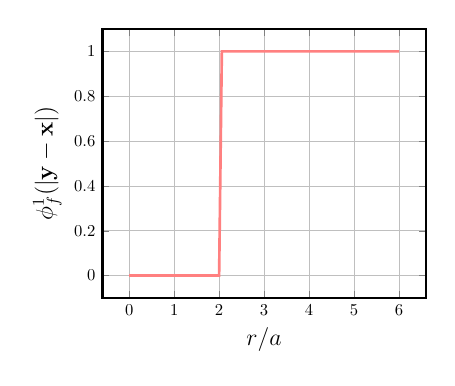
\begin{tikzpicture}[scale=0.6]
    \begin{axis}[
        xlabel={\Large$r/a$},
        ylabel={\Large$\phi_f^1(|\textbf{y}-\textbf{x}|)$},
        legend style={at={(0.05,0.05)}, anchor=south west},
        grid=major,
        domain=0:6,
        samples=100,
        ultra thick
    ]
    
    % Plot for phi = 0.05
    \addplot[color=red!50,ultra thick]
    { x < 2 ? 0 : 1};
    % \addlegendentry{$\phi = 0.05$}
    
    % % Plot for phi = 0.01
    % \addplot[color=blue!50,ultra thick]
    % { exp(-0.01 * (x^3 - 1))};
    % \addlegendentry{$\phi = 0.01$}
    
    % % Plot for phi = 0.001
    % \addplot[color=green!50,ultra thick]
    % { exp(-0.0001 * (x^3 - 1))};
    % \addlegendentry{$\phi = 10^{-4}$}
    
    \end{axis}
\end{tikzpicture}


In that case we must treat the problem into three region 
\paragraph*{First : $|\textbf{y} - \textbf{x}| > 2a$ :} we have $\phi_f^1 = \phi_f$, thus, $\phi_f^{1d} = 0$. same for $\phi_d$
\begin{align*}
    \avg{(\delta_1 - P_1)\rho^0\textbf{w}}
    &=0\\
    \avg{(\delta_1 - P_1)\rho^0\textbf{u}^0} / P_1
    &= 
    % \avg{(\delta_1 - P_1)\rho_f\chi_f\textbf{u}^0_f}
    % \avg{(\delta_1 - P_1)\rho_d\chi_d\textbf{u}^0_d}
    % = 
    \rho_f\phi_f\textbf{u}^{1d}_f
    + 
    \rho_d\phi_d\textbf{u}^{1d}_d
    \\
    \avg{(\delta_1 - P_1)\bm\sigma^0} 
    &= 
    - \phi_f^1 p^{1d}_f\bm\delta P_1 
    +\mu_f P_1 (\grad \textbf{u}^{1d} + \grad \textbf{u}^{1d})
    + \avg{(\delta_1 - P_1) \chi_d\bm\sigma^0_d}
\end{align*}
My guess is $\rho_f\phi_f\textbf{u}^{1d}_f
+ 
\rho_d\phi_d\textbf{u}^{1d}_d = \textbf{u}^{1d}$ 

and indeed we have 
\begin{equation*}
    \avg{\delta_1\textbf{u}^0} - \textbf{u}P_1
    = \avg{\delta_1 \chi_f \textbf{u}_f^0 + \chi_d \textbf{u}_d^0\delta_1 }
    - \textbf{u}_f\phi_fP_1
    - \textbf{u}_d\phi_dP_1
    \approx
    \phi_f^1 \textbf{u}_f^{1d} 
    + \phi_d^1 \textbf{u}_d^{1d}
\end{equation*}

\subsubsection*{Computation of the fluid phase term}

For suspension of spherical particles in the dilute limit the fluid phase averaged fields may be simplyfied by noticing that $\phi_f^1[\textbf{x},t;\textbf{y},\textbf{c}] P_1[\textbf{y},\textbf{c},t] = P_1[\textbf{y},\textbf{c},t]$ when $|\textbf{x} - \textbf{y}| > a$. 
\begin{equation}
    \avg{\chi_f f_f^0}[\textbf{x},t]
    = 
    \int_{\mathbb{R}^3}
    \int_{\mathbb{R}^3}
    f_f^1 \phi_f^1[\textbf{x},t;\textbf{y},\textbf{c}] P_1[\textbf{y},\textbf{c},t]
    d\textbf{y} 
    d\textbf{c}
\end{equation}
where,
\begin{equation*}
    f_f^1 \phi_f^1[\textbf{x},t;\textbf{y},\textbf{c}] P_1[\textbf{y},\textbf{c},t]
    =     
    \int
    \frac{1}{N}
    \sum_\alpha \delta(\textbf{y}-\textbf{x}_\alpha)
     \delta(\textbf{c}-\textbf{u}_\alpha)
    \chi_f
    f^0_f[\textbf{x},t;\FF]
    d\PP.
\end{equation*}
